\documentclass[aspectratio=169]{beamer}

% Theme and color scheme
\usetheme{Madrid}
\usecolortheme{default}

% Packages
\usepackage[utf8]{inputenc}
\usepackage[T1]{fontenc}
\usepackage{graphicx}
\usepackage{listings}
\usepackage{xcolor}
\usepackage{tikz}
\usepackage{booktabs}
\usepackage{multicol}

% Code listing setup
\lstset{
    basicstyle=\tiny\ttfamily,
    breaklines=true,
    frame=single,
    backgroundcolor=\color{gray!10},
    keywordstyle=\color{blue},
    commentstyle=\color{green!60!black},
    stringstyle=\color{red}
}

% Title information
\title[AI for Menopause Education]{Breaking the Silence: Large Language Models for\\Culturally-Sensitive Menopause Education}
\subtitle{AI Ethics, Cultural Sensitivity \& Health Informatics}
\author{Student Team Presentation}
\institute{Computer Science Department}
\date{\today}

% Custom colors
\definecolor{primarycolor}{RGB}{0, 102, 153}
\definecolor{secondarycolor}{RGB}{153, 0, 102}
\definecolor{accentcolor}{RGB}{255, 153, 0}

\begin{document}

% Title slide
\begin{frame}
    \titlepage
\end{frame}

% Table of contents
\begin{frame}{Outline}
    \tableofcontents
\end{frame}

\section{Project Overview}

\begin{frame}{Assignment Summary}
    \begin{block}{Core Objective}
        Design and develop a culturally-sensitive AI system for menopause education, addressing global health education gaps through personalized Large Language Model applications.
    \end{block}
    
    \begin{columns}[t]
        \begin{column}{0.5\textwidth}
            \textbf{Key Topics:}
            \begin{itemize}
                \item Large Language Models
                \item AI Ethics \& Safety
                \item Cultural AI
                \item Health Informatics
                \item Bias Detection
                \item Human-Computer Interaction
            \end{itemize}
        \end{column}
        \begin{column}{0.5\textwidth}
            \textbf{Target Audience:}
            \begin{itemize}
                \item High School Students (Grades 9-12)
                \item CS1 College Students
            \end{itemize}
            
            \textbf{Timeline:}
            \begin{itemize}
                \item Phase 1: 2-3 weeks (Research/Design)
                \item Phase 2: 3-4 weeks (Implementation)
                \item \textbf{Total: 5-7 weeks}
            \end{itemize}
        \end{column}
    \end{columns}
\end{frame}

\begin{frame}{Project Strengths \& Challenges}
    \begin{columns}[t]
        \begin{column}{0.5\textwidth}
            \begin{block}{Strengths}
                \begin{itemize}
                    \item Addresses real-world health equity issues
                    \item Combines technical skills with social impact
                    \item Teaches AI ethics through practical application
                    \item Culturally inclusive and globally relevant
                    \item Integrates multiple AI concepts
                \end{itemize}
            \end{block}
        \end{column}
        \begin{column}{0.5\textwidth}
            \begin{alertblock}{Challenges}
                \begin{itemize}
                    \item Requires sensitive handling of health topics
                    \item Cultural research requires substantial time
                    \item Technical implementation requires programming experience
                    \item May be challenging without health background
                \end{itemize}
            \end{alertblock}
        \end{column}
    \end{columns}
\end{frame}

\section{Phase 1: Research \& Design}

\begin{frame}{Phase 1: Understanding the Global Crisis}
    \begin{block}{Objective}
        Understand the global menopause education crisis and design a culturally-sensitive AI solution
    \end{block}
    
    \begin{columns}[t]
        \begin{column}{0.6\textwidth}
            \textbf{Research Areas:}
            \begin{itemize}
                \item Global menopause education gaps
                \item Cultural perspectives on menopause
                \item Current AI applications in health
                \item Ethical considerations
                \item Technical feasibility assessment
            \end{itemize}
        \end{column}
        \begin{column}{0.4\textwidth}
            \textbf{Deliverables:}
            \begin{itemize}
                \item Literature review
                \item Cultural analysis
                \item System design proposal
                \item Ethics framework
            \end{itemize}
        \end{column}
    \end{columns}
\end{frame}

\begin{frame}{Cultural Assessment Framework}
    \begin{block}{Core Concept}
        Different cultures view menopause differently - from "liberation" to "medical condition" to neutral transition
    \end{block}
    
    \begin{table}
        \centering
        \small
        \begin{tabular}{|l|l|l|}
            \hline
            \textbf{Liberation View} & \textbf{Medical View} & \textbf{Neutral View} \\
            \hline
            Freedom \& wisdom & Condition requiring treatment & Normal life stage \\
            Empowerment focus & Symptom management & Balanced information \\
            Traditional communities & Urban/modern lifestyle & Mixed influences \\
            Community guidance & Professional medical advice & Independent learning \\
            \hline
        \end{tabular}
    \end{table}
    
    \textbf{Key Insight:} AI system must adapt content based on user's cultural perspective
\end{frame}

\section{Phase 2: Technical Implementation}

\begin{frame}{Phase 2: System Architecture}
    \begin{block}{Objective}
        Build a working prototype of the AI-powered menopause education system
    \end{block}
    
    \begin{center}
        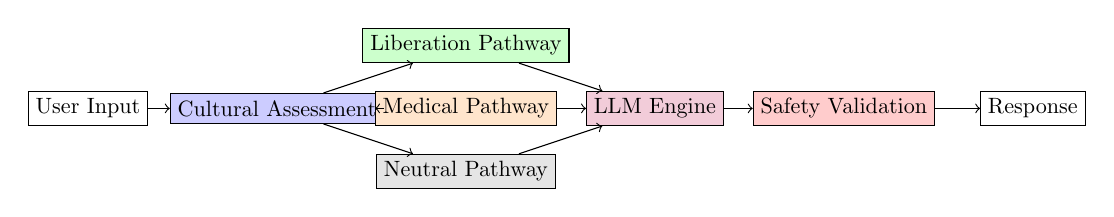
\begin{tikzpicture}[scale=0.8, every node/.style={scale=0.8}]
            % Input
            \node[draw, rectangle] (input) at (0,0) {User Input};
            
            % Cultural Assessment
            \node[draw, rectangle, fill=blue!20] (assessment) at (3,0) {Cultural Assessment};
            
            % Pathways
            \node[draw, rectangle, fill=green!20] (liberation) at (6,1) {Liberation Pathway};
            \node[draw, rectangle, fill=orange!20] (medical) at (6,0) {Medical Pathway};
            \node[draw, rectangle, fill=gray!20] (neutral) at (6,-1) {Neutral Pathway};
            
            % LLM Engine
            \node[draw, rectangle, fill=purple!20] (llm) at (9,0) {LLM Engine};
            
            % Safety Layer
            \node[draw, rectangle, fill=red!20] (safety) at (12,0) {Safety Validation};
            
            % Output
            \node[draw, rectangle] (output) at (15,0) {Response};
            
            % Arrows
            \draw[->] (input) -- (assessment);
            \draw[->] (assessment) -- (liberation);
            \draw[->] (assessment) -- (medical);
            \draw[->] (assessment) -- (neutral);
            \draw[->] (liberation) -- (llm);
            \draw[->] (medical) -- (llm);
            \draw[->] (neutral) -- (llm);
            \draw[->] (llm) -- (safety);
            \draw[->] (safety) -- (output);
        \end{tikzpicture}
    \end{center}
\end{frame}

\begin{frame}[fragile]{Content Routing System}
    \begin{block}{Adaptive Content Delivery}
        System routes users to appropriate content pathways based on cultural assessment
    \end{block}
    
    \begin{lstlisting}[language=Python, caption=Content Router Implementation]
class ContentRouter:
    def __init__(self):
        self.pathways = {
            "liberation": LiberationPathway(),
            "medical": MedicalPathway(),
            "neutral": NeutralPathway()
        }
    
    def route_user(self, assessment_results):
        """Route user to appropriate content pathway"""
        score = self.calculate_pathway_score(assessment_results)
        return self.pathways[score["dominant_pathway"]]
    \end{lstlisting}
\end{frame}

\begin{frame}[fragile]{Safety Validation Layer}
    \begin{alertblock}{Critical Component}
        Multi-layered safety validation to prevent misinformation and ensure cultural sensitivity
    \end{alertblock}
    
    \begin{lstlisting}[language=Python, caption=Safety Validator]
class SafetyValidator:
    def validate_response(self, response, user_context):
        """Multi-layer safety validation"""
        medical_check = self.verify_medical_accuracy(response)
        bias_check = self.detect_cultural_bias(response, user_context)
        confidence_check = self.assess_confidence(response)
        content_check = self.validate_content_appropriateness(response)
        
        return {
            "approved": all([medical_check, bias_check, 
                           confidence_check, content_check]),
            "requires_human_review": not medical_check,
            "safety_flags": self.get_safety_flags(response)
        }
    \end{lstlisting}
\end{frame}

\begin{frame}{Bias Detection Framework}
    \begin{block}{Identifying Cultural Bias}
        System monitors for various types of bias in AI responses
    \end{block}
    
    \begin{table}
        \centering
        \footnotesize
        \begin{tabular}{|l|l|c|}
            \hline
            \textbf{Bias Type} & \textbf{Description} & \textbf{Weight} \\
            \hline
            Western Centrism & Imposing universal standards & 0.8 \\
            Medical Bias & Pathologizing natural experiences & 0.9 \\
            Age Bias & Negative framing of aging & 0.7 \\
            Gender Bias & Stereotypical assumptions & 0.9 \\
            Socioeconomic Bias & Assuming expensive treatments & 0.6 \\
            \hline
        \end{tabular}
    \end{table}
    
    \textbf{Key Features:}
    \begin{itemize}
        \item Real-time bias scoring
        \item Cultural appropriateness assessment
        \item Automated bias reduction recommendations
    \end{itemize}
\end{frame}

\section{Assessment \& Evaluation}

\begin{frame}{Assessment Rubric}
    \begin{table}
        \centering
        \tiny
        \begin{tabular}{|p{1.8cm}|p{1.8cm}|p{1.8cm}|p{1.8cm}|p{1.8cm}|c|}
            \hline
            \textbf{Component} & \textbf{Excellent (90-100\%)} & \textbf{Good (80-89\%)} & \textbf{Satisfactory (70-79\%)} & \textbf{Needs Improvement (<70\%)} & \textbf{Weight} \\
            \hline
            Research Quality & Comprehensive research with diverse sources & Good research with credible sources & Adequate research & Limited research & 20\% \\
            \hline
            Technical & Fully functional system & Mostly functional with minor bugs & Basic functionality & Major functionality missing & 25\% \\
            \hline
            Cultural Sensitivity & Exceptional cultural awareness & Good cultural consideration & Basic awareness & Little cultural consideration & 20\% \\
            \hline
            AI Ethics \& Safety & Comprehensive safety mechanisms & Good safety considerations & Basic safety measures & Inadequate safety & 20\% \\
            \hline
            Presentation & Clear, engaging presentation & Good presentation & Adequate presentation & Poor communication & 15\% \\
            \hline
        \end{tabular}
    \end{table}
\end{frame}

\section{Implementation Variants}

\begin{frame}{Project Variants}
    \begin{columns}[t]
        \begin{column}{0.5\textwidth}
            \begin{block}{Simplified Version}
                \textbf{For Beginners:}
                \begin{itemize}
                    \item Focus only on Phase 1 research and design
                    \item No technical implementation required
                    \item Emphasis on cultural understanding
                    \item Paper prototype development
                \end{itemize}
            \end{block}
            
            \begin{block}{Advanced Version}
                \textbf{For Experienced Students:}
                \begin{itemize}
                    \item Implement machine learning models for bias detection
                    \item Advanced NLP techniques
                    \item Real API integrations
                    \item User testing and evaluation
                \end{itemize}
            \end{block}
        \end{column}
        \begin{column}{0.5\textwidth}
            \begin{block}{Cross-Curricular}
                \textbf{Interdisciplinary Approach:}
                \begin{itemize}
                    \item Partner with health/biology classes
                    \item Collaborate with social studies
                    \item Include psychology perspectives
                    \item Medical professional interviews
                \end{itemize}
            \end{block}
            
            \begin{block}{Global Perspective}
                \textbf{International Scope:}
                \begin{itemize}
                    \item Compare multiple cultural contexts
                    \item Beyond India - explore other cultures
                    \item Cross-cultural validation
                    \item Global health equity analysis
                \end{itemize}
            \end{block}
        \end{column}
    \end{columns}
\end{frame}

\section{Dependencies \& Prerequisites}

\begin{frame}{Prerequisites \& Dependencies}
    \begin{columns}[t]
        \begin{column}{0.5\textwidth}
            \begin{block}{High School Level}
                \textbf{Required:}
                \begin{itemize}
                    \item Basic understanding of AI concepts
                    \item Internet research skills
                    \item Presentation abilities
                    \item Cultural sensitivity awareness
                \end{itemize}
                
                \textbf{Helpful:}
                \begin{itemize}
                    \item Basic programming exposure
                    \item Health science background
                \end{itemize}
            \end{block}
        \end{column}
        \begin{column}{0.5\textwidth}
            \begin{block}{CS1 College Level}
                \textbf{Required:}
                \begin{itemize}
                    \item Python programming fundamentals
                    \item Basic web technologies (HTML/CSS)
                    \item Introduction to APIs
                    \item Data structures knowledge
                \end{itemize}
                
                \textbf{Helpful:}
                \begin{itemize}
                    \item Machine learning basics
                    \item Database concepts
                    \item UI/UX design principles
                \end{itemize}
            \end{block}
        \end{column}
    \end{columns}
\end{frame}

\section{Conclusion}

\begin{frame}{Key Learning Outcomes}
    \begin{block}{Students Will Learn:}
        \begin{multicols}{2}
            \begin{itemize}
                \item AI ethics in healthcare
                \item Cultural sensitivity in technology
                \item Bias detection and mitigation
                \item LLM applications and limitations
                \item Health informatics principles
                \item Human-computer interaction
                \item Safety-critical system design
                \item Global health equity issues
                \item Research and analysis skills
                \item Technical implementation
                \item Presentation and communication
                \item Interdisciplinary collaboration
            \end{itemize}
        \end{multicols}
    \end{block}
\end{frame}

\begin{frame}{Project Impact}
    \begin{center}
        \Large
        \textcolor{primarycolor}{\textbf{Breaking the Silence}}
        
        \vspace{1em}
        
        This project addresses a real-world health crisis affecting over 1 billion women globally while teaching cutting-edge AI concepts through practical, ethical application.
        
        \vspace{1em}
        
        \textcolor{secondarycolor}{\textbf{Technology + Ethics + Cultural Sensitivity = Real Impact}}
    \end{center}
    
    \begin{alertblock}{Remember}
        Success depends not just on technical implementation, but on cultural understanding, ethical considerations, and commitment to health equity.
    \end{alertblock}
\end{frame}

\begin{frame}
    \begin{center}
        \Huge Thank You!
        
        \vspace{2em}
        
        \Large Questions \& Discussion
        
        \vspace{1em}
        
        \normalsize
        \textit{"AI can break the silence, but only with wisdom, ethics, and cultural respect."}
    \end{center}
\end{frame}

\end{document}
